\documentclass[11pt,a4paper]{article}

\usepackage[utf8]{inputenc} 
\usepackage[T1]{fontenc} 
\usepackage{lmodern}
\usepackage[margin=2cm]{geometry}
\usepackage[german]{babel}
\usepackage{array}
\setlength{\parindent}{0pt}
\setlength{\parskip}{1ex plus 0.5ex minus 0.5ex}

\usepackage{amsmath} 
\usepackage{graphicx} 
\usepackage{booktabs}
\usepackage[colorlinks]{hyperref}
\usepackage{nicefrac}
\usepackage{gensymb}
\usepackage[usenames,dvipsnames,svgnames,table]{xcolor}
\usepackage{multirow}
\usepackage{tikz}

\hbadness=99999

\newcommand{\refpy}[1]{Siehe Anhang: \textit{Rechnungen in Python} (\texttt{{\color{incolor}In [{\color{incolor}#1}]}})}
\newcommand\dif{\mathop{}\!\mathrm{d}}
\newcommand{\halftime}[4]{\begin{figure}[h]
\begin{minipage}{.#1\textwidth}#3\end{minipage}\begin{minipage}{.#2\textwidth}
\centering
#4\end{minipage}
\end{figure}}
\renewcommand{\vec}{\boldsymbol}

\usepackage{etoolbox}

\makeatletter
\patchcmd{\@classz}
  {\CT@row@color}
  {\oldCT@column@color}
  {}
  {}
\patchcmd{\@classz}
  {\CT@column@color}
  {\CT@row@color}
  {}
  {}
\patchcmd{\@classz}
  {\oldCT@column@color}
  {\CT@column@color}
  {}
  {}
\makeatother

\begin{document}

{
\centering 
\large 
Physiklabor für Anf\"anger*innen \\
Ferienpraktikum im Sommersemester 2018 \\[4mm]
\textbf{\LARGE 
Versuch 17: Trägheitsmomente/Steinerscher Satz
} \\[3mm]
(durchgef\"uhrt am 17.09.2018 bei Adrian Hauber)\\
Gruppe 14: Andréz Gockel, Patrick M\"unnich\\ 
\today \\[10mm]
}

\section{Ziel des Versuchs}

Dieser Versuch hat zwei Teile. Im ersten Teil wird mit Hilfe von einer hergeleiteten Formel (\ref{}), die den Trägheitsmoment mit der Periodendauer in Zusammenhang bringt das Trägheitsmoment eines ausgedehnten starren Körper berechnet. Dieses wird verglichen mit dem experimentell bestimmten Wert. Das Trägheitsmoment wird bestimmt von einer zylindrische Stange, die nicht im Schwerpunkt aufgehängt wird und die per hand in Schwingung versetzt wird, in dem die Schwingungsdauer gemessen wird und den Wert mit der hergeleiteten Formel berechnet wird. In dem zweiten Teil wird von einem Drehpendel den Zusammenhang von der Schwingungsdauer und dem Abstand von einer Zusatzmasse zum Mittelpunkt verwendet, um hiermit den Steinerschen Satz experimentell zu verifizieren. 

\section{Teil 1 - Trägheitsmomente}
\subsection{Herleitung der Schwingungsgelichung}

Der unterschied von einem mathematischen Pendel und einem physikalischen Pendels ist dass, es sich nicht um eine punktförmige Masse handelt sondern den Schwerpunkt von einem starren Körper wo das Trägheitsmoment berücksichtigt werden muss. Mit der rücktreibenden Kraft $F_r = mg\sin\varphi$ und den Abstand von Aufhängepunkt zu Schwerpunkt $d$ können wir das Drehmoment ausdrücken als:
$$\vec{M} = \vec{F_r} \times \vec{d} = dm\vec{g}\sin(\varphi)$$
mit der klein Winkel Näherung: $\sin\varphi \approx \varphi$:
$$\vec{M} = dm\vec{g}\varphi$$
Dies wird gleichgesetzt mit:
$$\vec{M} = \vec{\dot L} = - I \cdot \vec{\dot\omega} = - I \cdot \ddot \varphi$$
$$\Rightarrow - I \cdot \ddot \varphi = dm\vec{g}\varphi \quad \Rightarrow \ddot \varphi = - \bigg(\underbrace{\frac{dm\vec{g}}{I}}_{\omega^2}\bigg)\varphi \quad \Rightarrow \ddot \varphi = - \omega^2 \varphi$$
Mit $T = 2\pi \frac{1}{\vec{\omega}}$ bekommt man: $T = 2\pi \sqrt{\frac{I}{dm\vec{g}}}$.

Zunächst wird das Trägheitsmoment eines starren Körpers, in diesem fall einen Vollzylinder berechnet. Allgemein für das Trägheitsmoment bezüglich der Drehachse gilt:
$$I = \int \vec{r}^2 \dif m$$
mit $m = \rho V$ und angenommen der Zylinder ist homogen bekommt man: $\displaystyle{I = \rho \int_V \vec{r}^2 \dif V}$

in Zylinderkoordinaten: $\vec{r}^2 = $
$$I = \rho \int\displaylimits_{0}^{2\pi} \int\displaylimits_{0}^{l}\int\displaylimits_{0}^{r}\dif\phi \dif z \dif r$$ 
wobei 
\subsection{Aufbau}
\halftime{5}{5}{Ein zylindrischer Stab der an einem Stativ gehängt werden kann. Zusätzlich wird benötigt ein Bandmass, Messschieber und eine Stoppuhr für die Messungen. }{
\centering
\fbox{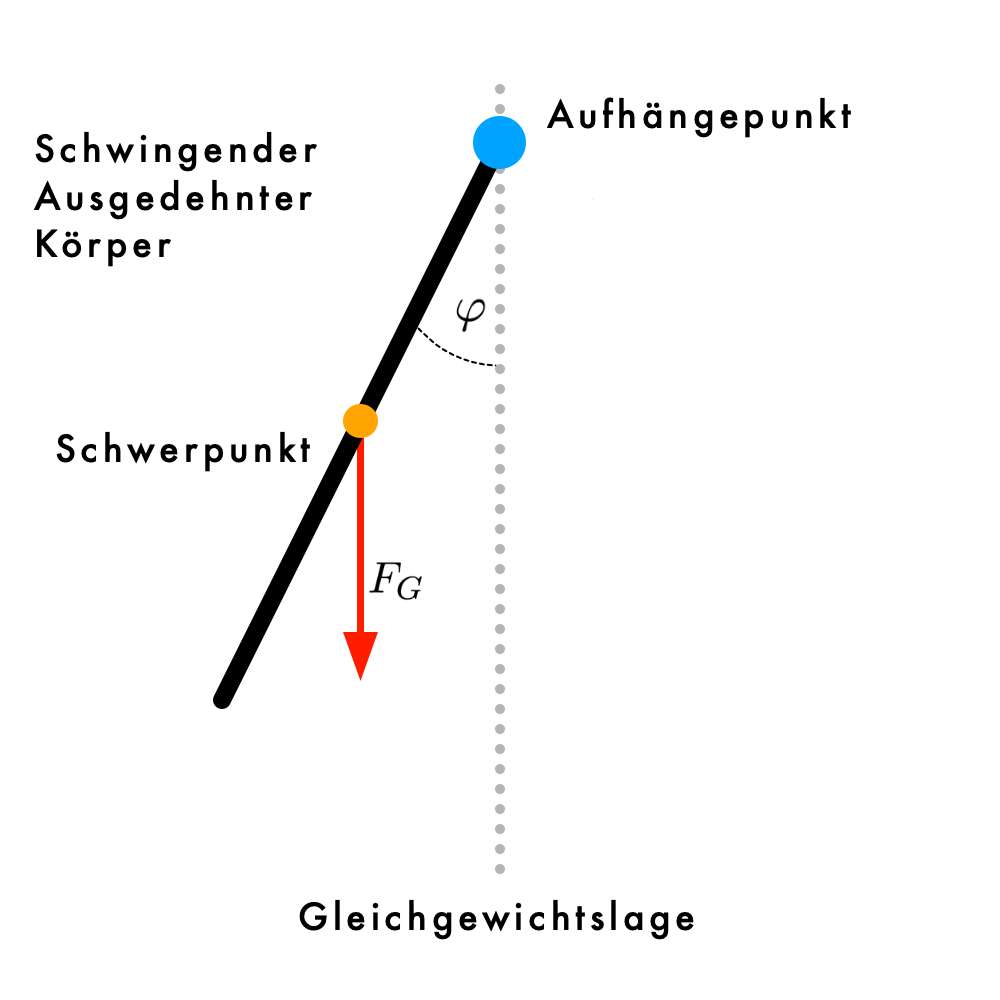
\includegraphics[width=0.5\textwidth]{Spend}}
   \renewcommand\thefigure{B1}
\caption{Versuchsaufbau}
\label{JS1}
}

\subsection{Durchführung}

Zuerst wurde die Länge des Stabes mittels Bandmass gemißt. Zunächst wurde mittels Messschieber der Durchmesser des Stabes gemißt. Dann wurde der Stab and das Stativ gehängt und per hand zum pendeln gebracht. Es wurde mit der Stoppuhr 30 mal eine Periode zeitlich gemessen. Danach wurde ein mal 30 Perioden gemißt, um zu schauen welches verfahren ein kleineren Fehler hat. Dies ergab sich als das zweite verfahren. 

\subsubsection{Auswertung}

$$
\begin{array}{lc}
	\multicolumn{1}{l}{\textrm{Zu Bestimmende Werte}} \\
	\toprule 
	\textrm{Stablänge} & l = 95.6(3)\,\textrm{cm} \\
	\textrm{Radius} & r = 5.0(2)\,\textrm{mm} \\
	\bottomrule 
\end{array}
$$


\pagebreak

\subsection{Teil B - Umwandlung von elektrischer Arbeit in Wärme}

\subsubsection{Aufgabenstellung}

Zur Bestimmung der W\"armekapazit\"at durch Umwandlung von elektrischer Arbeit in W\"arme nutzt man ein Kalorimeter mit einem Widerstand und Thermometer. Zum Aufw\"armen des Wassers wird der Widerstand an eine Spannungsquelle angeschlo\ss en. Die Temperatur\"anderung wird dann bis zu einem beliebigen Punkt abschnittsweise gemessen. Danach wird gemessen, ab welchem Zeitpunkt die Temperatur wieder abf\"allt.

\subsubsection{Auswertung}

$$
\begin{array}{lc}
	\multicolumn{1}{l}{\textrm{Zu Bestimmende Werte}} \\
	\toprule 
	\textrm{Stablänge} & l = 95.6(3)\,\textrm{cm} \\
	\textrm{Radius} & r = 5.0(2)\,\textrm{mm} \\
	\bottomrule \\
	\multicolumn{2}{l}{\textrm{Bekannte Werte}} \\
	\toprule
	\textrm{Volumen des Glaskolbens} & V = (2225 \pm 5)\,\textrm{cm}^3\\
	\bottomrule 
\end{array}
$$

Es wurden zwei Messungen durchgef\"uhrt mit jeweils $116.94\,$g und $113.42\,$g Wasser. Die Wassermenge wurde so gew\"ahlt, damit der Widerstand und das Thermometer in dem Wasser eingetaucht sind. Die Dauern der Messungen waren 38 und 20 Minuten. Diese wurden so gew\"ahlt, dass sie m\"oglichst kurz ausfallen sollten. Temperatur\"anderungen wurden im Abstand von 60 Sekunden gemessen, da diese sonst nicht auff\"allig genug w\"aren, um etwas zu erkennen. Die Messwerte hierzu sind aufgrund ihrer L\"ange im Anhang.

Das extrapolationsverfahren der 1. Messreihe ergibt $T_{max} = 26.5\celsius$ da der Temperaturabfall erst nach 30 begann. Für die 2. Messreihe ergibt das extrapolationsverfahren $T_{max} = 41.45\celsius$ \ref{Dia:1}, \ref{Dia:2}, \ref{Ext}

\begin{table}[h!]
	\centering
	\rowcolors{2}{gray!10}{white}
	\begin{tabular}{|c|cccc|}
		\multicolumn{5}{c}{\textrm{Extrapolationverfahren}} \\
		\noalign{\global\arrayrulewidth=0.4mm}
		\hline
		\noalign{\global\arrayrulewidth=0.2mm}
		\textrm{Messreihe} & $a$ in \celsius & $u_a$ in \celsius & b in $\nicefrac{\celsius}{\textrm{s}}$ & $u_b$ in $\nicefrac{\celsius}{\textrm{s}}$ \\
		\hline
	1 & 26.5 & 0.037 &  -33.579 & 2.105 $\times 10^{-5}$ \\
	2 & 42.65 & 1.605 & -0.0025 & 0.001443 \\
		\hline
	\end{tabular}
	\renewcommand\thetable{T3}
	\caption{Wertetabelle für die extrapolation}
	\label{Ext}
\end{table}

Uns ist bekannt, dass $W_{el}$ vollst\"andig in W\"armeenergie, $Q$, umgewandelt wird. Folgende Formeln gelten:

\begin{equation}
Q=(C_{Kal}+m_wc_w)\Delta T\label{Q_el}
\end{equation}
\begin{equation}
W_{el}=\int P\mathrm{d}t=\int UI\mathrm{d}t.
\end{equation}

Da $P$ konstant ist, kann man hier einfach mit

\begin{equation}
W_{el}=UI\Delta t\label{W_el}
\end{equation}

rechnen. Bei unserer Messreihe waren die werte f\"ur $U$ und $I$ jeweils 14.9\,V und 1.5\,A.\\

Stellen wir (\ref{Q_el}) nach $c_w$ um und setzen (\ref{W_el}) ein, so bekommen wir als Formel:

\begin{equation}
c_w=\frac{UI\frac{\Delta t}{\Delta T}-C_{Kal}}{m_w}.
\end{equation}

Unser $m_w$, die Masse des Wassers, ist wie oben erw\"ahnt bei der ersten Messreiehe $116.94(3)\,$g und bei der zweiten $113.42(3)\,$g. Somit ergeben unsere Werte f\"ur $c_w$:

\begin{table}[h!]
	\centering
	\rowcolors{2}{gray!10}{white}
	\begin{tabular}{|c|cccc|}
		\noalign{\global\arrayrulewidth=0.4mm}
		\hline
		\noalign{\global\arrayrulewidth=0.2mm}
		\textrm{Messung} & $1$ & $2$  & Mittelwert & Gewichtet\\
		\hline
	\textrm{W\"armekapazit\"at} $\left[\mathrm{\nicefrac{\mathrm{J}}{kg K}}\right]$ & $7330\pm0.09$ & $8790\pm0.11$ & $8060\pm0.10$ & $7931\pm0.07$ \\		
	\hline
	\end{tabular}
	\renewcommand\thetable{T3}
	\caption{Wertetabelle W\"armekapazit\"at}
	\label{Ext}
\end{table}

Der gewichtete arithmetische Mittelwert wurde gleich wie beim ersten Teil berechnet. Mit der Formel f\"ur die Abweichung aus Teil A, (\ref{abw}), sind wir hier $t = 53543$ von dem Literaturwert entfernt.\\

Der gro\ss e Unterschied zwischen den Abweichungen liegt vermutlich dabei, dass beim zweiten Versuch man wesentlich ungenauer ablesen musste. Dieses Problem ist durch die kurze Erw\"armungsphase vergr\"o\ss ert wordene. H\"atte man zu einer h\"oheren Temperatur erw\"armt, so w\"urde es sich auch schneller abk\"uhlen und man k\"onnte einen gr\"o\ss eren Temperaturabstand als Indikator f\"ur das Senken der Temperatur w\"ahlen.\\

Au\ss erdem haben wir noch einen systematischen Fehler aufgrund des R\"uhrens des Wassers, was zur Mischung dient, aber wodurch kinetische Energie hinzugef\"ugt wird, welches das Wasser auch aufw\"armt. Dazu kann man noch erw\"ahnen, dass die Au\ss entemperatur steigt, wodurch das Wasser nicht immer gleich abk\"uhlt. Dies ist jedoch aufgrund der kurzen Dauer der Messung nicht sehr einflussreich.

\vfill

\begin{thebibliography}{9}
 \bibitem{Uncertainties}''Correlations between variables are automatically handled, which sets this module apart from many existing error propagation codes.'' - https://pythonhosted.org/uncertainties/
 \end{thebibliography}
%Systematische und statistische Fehler.

\pagebreak


\section{Anhang}




\begin{table}[h]
	\centering
	\rowcolors{2}{gray!10}{white}
	\begin{tabular}{|r|l|}
		\multicolumn{2}{c}{\textrm{Messreihe 1}} \\
		\noalign{\global\arrayrulewidth=0.4mm}
		\hline
		\noalign{\global\arrayrulewidth=0.2mm}
		\textrm{Rotationen }$n \pm 0.3$ & \textrm{Temperatur }$T \pm 0.05\celsius$\\
		\hline
		0 & 24 \\
		10 & 24.1 \\
		20 & 24.3 \\
		30 & 24.5 \\
		40 & 24.6 \\
		50 & 24.8 \\
		\hline
	\end{tabular}
	\renewcommand\thetable{T1}
	\caption{Messreihe 1 für Teil A}
	\label{table:m1}
\end{table}

\begin{table}[h]
	\centering
	\rowcolors{2}{gray!10}{white}
	\begin{tabular}{|r|l|}
		\multicolumn{2}{c}{\textrm{Messreihe 2}} \\
		\noalign{\global\arrayrulewidth=0.4mm}
		\hline
		\noalign{\global\arrayrulewidth=0.2mm}
		\textrm{Rotationen }$n \pm 0.3$ & \textrm{Temperatur }$T \pm 0.05\celsius$\\
		\hline
		0 & 24.3 \\
		5 & 24.3 \\
		10 & 24.4 \\
		15 & 24.5 \\
		20 & 24.6 \\
		25 & 24.7 \\
		30 & 24.8 \\
		35 & 24.9 \\
		40 & 25 \\
		45 & 25.1 \\
		50 & 25.2 \\
		55 & 25.2 \\
		60 & 25.4 \\
		65 & 25.5 \\
		70 & 25.5 \\
		75 & 25.6 \\
		80 & 25.6 \\
		85 & 25.7 \\
		90 & 25.8 \\
		95 & 26 \\
		100 & 26 \\
		\hline
	\end{tabular}
	\renewcommand\thetable{T2}
	\caption{Messreihe 2 für Teil A}
	\label{table:m2}
\end{table}

\begin{table}[h]
\centering
\rowcolors{2}{gray!10}{white}
\begin{tabular}{|>{\columncolor[gray]{1}}c|r|r|r|}
\multicolumn{2}{c}{}&\multicolumn{1}{c}{Luft} & \multicolumn{1}{c}{Argon}\\
\hline
Messreihe & Periode & Zeit in $s$ & Zeit in $s$\\
\hline 
&200$\pm14$  & 78.53  &  75.06 \\
&400$\pm20$  & 156.89 & 149.50 \\
&600$\pm25$  & 235.78 & 223.57 \\
&800$\pm28$  & 314.35 & 297.25 \\
\multirow{-5}{*}{1}
&1000$\pm32$ & 392.34 & 370.68 \\ 
\hline
&200$\pm14$  & 78.44  &  73.03 \\
&400$\pm20$  & 156.87 & 145.91 \\
&600$\pm25$  & 235.38 & 218.79 \\
&800$\pm28$  & 313.95 & 291.47 \\
\multirow{-5}{*}{2}
&1000$\pm32$ & 392.52 & 364.06 \\ 
\hline
&100$\pm10$ & 39.09 & 36.10 \\
&100$\pm10$ & 38.96 & 36.18 \\
&100$\pm10$ & 39.16 & 36.14 \\
&100$\pm10$ & 39.00 & 36.10 \\
\multirow{-5}{*}{3}
&100$\pm10$ & 39.96 & 36.16 \\ 
\hline
\end{tabular}
\renewcommand\thetable{T1}
\caption{1. Messwerte}
\label{tab:B1}
\end{table}

\begin{table}[h]
\centering
$\begin{array}{rl}
\multicolumn{2}{l}{\textrm{\underline{Unsicherheiten:}}}\\
\textrm{Zeit: } & \pm 0.03 \textrm{s}\\
\textrm{Temperatur: } & \pm 0.02 \textrm{\celsius}\\
\textrm{Strom: } & \pm 0.018 \textrm{A}\\
\textrm{Spannung: } & \pm 0.12 \textrm{V}
\end{array}$
\rowcolors{2}{gray!10}{white}
\begin{tabular}{|c|c|c|c|}
\multicolumn{4}{l}{Wasser 113.42(3)\,g}\\
\hline
$t$ in s & $T$ in $^\circ\textrm{C}$ & $I$ in A & $U$ in V \\
\hline 
0   & 22 & 1.5 & 14.9\\
60  & 22 & 1.5 & 14.9\\
120 & 23 & 1.5 & 14.9\\
180 & 24 & 1.5 & 14.9\\
240 & 26 & 1.5 & 14.9\\ 
300 & 27 & 1.5 & 14.9\\ 
360 & 28 & 1.5 & 14.9\\ 
420 & 29.2 & 1.5 & 14.9\\ 
480 & 30.3 & 1.5 & 14.9\\ 
540 & 31.9 & 1.5 & 14.9\\ 
600 & 33 & 1.5 & 14.9\\ 
660 & 33.7 & 1.5 & 14.9\\ 
720 & 35 & 1.5 & 14.9\\ 
780 & 35 & 1.5 & 14.9\\ 
840 & 36 & 1.5 &14.9\\
900 & 37 & 1.5 & 14.9\\
960 & 38.2 & 0 & 0\\
1020 & 39.5 & 0 & 0\\
1080 & 40 & 0 & 0\\
1140 & 40 & 0 & 0\\
1200 & 39.5 & 0 & 0\\
\hline
\end{tabular}
\phantom{$\begin{array}{rl}
\multicolumn{2}{l}{\textrm{\underline{Unsicherheiten:}}}\\
\textrm{Zeit: } & \pm 0.03 \textrm{s}\\
\textrm{Temperatur: } & \pm 0.02 \textrm{\celsius}\\
\textrm{Strom: } & \pm 0.018 \textrm{A}\\
\textrm{Spannung: } & \pm 0.12 \textrm{V}
\end{array}$
}
\renewcommand\thetable{T5}
\caption{2. Messwerte für Teil B}
\label{tab:B2}
\end{table}

\pagebreak

\pagebreak
\phantom{lol}
\end{document}